\documentclass[tikz,border=12pt]{standalone}
\usepackage{tikz}
\usetikzlibrary{shapes.geometric, shapes.misc, arrows.meta, positioning, fit, backgrounds, calc}

\definecolor{clcblue}{RGB}{52, 101, 164}
\definecolor{wikigreen}{RGB}{34, 139, 34}
\definecolor{osmred}{RGB}{180, 50, 30}
\definecolor{llmviolet}{RGB}{100, 50, 160}
\definecolor{metricgold}{RGB}{180, 130, 0}
\definecolor{filtergray}{RGB}{90, 90, 90}
\definecolor{diagcyan}{RGB}{30, 120, 140}
\definecolor{boxbg}{RGB}{245, 247, 252}
\definecolor{arrowcol}{RGB}{60, 60, 80}
\definecolor{gemmaorange}{RGB}{205, 110, 35}

\tikzset{
  nohyphen/.style={execute at begin node={\hyphenpenalty=10000\exhyphenpenalty=10000}},
  datasrc/.style={
    nohyphen,
    rectangle, rounded corners=4pt,
    draw=#1!72!black, fill=#1!12,
    text width=3.10cm, align=center,
    font=\sffamily\footnotesize,
    inner sep=5pt, minimum height=1.05cm
  },
  process/.style={
    nohyphen,
    rectangle, rounded corners=3pt,
    draw=#1!80!black, fill=#1!10,
    text width=3.5cm, align=center,
    font=\sffamily\scriptsize,
    inner sep=4.5pt, minimum height=0.95cm
  },
  wideprocess/.style={
    nohyphen,
    rectangle, rounded corners=3pt,
    draw=#1!80!black, fill=#1!10,
    text width=3.90cm, align=center,
    font=\sffamily\scriptsize,
    inner sep=4.5pt, minimum height=0.95cm
  },
  taskbox/.style={
    nohyphen,
    rectangle, rounded corners=4pt,
    draw=#1!80!black, fill=#1!10,
    text width=3.80cm, align=center,
    font=\sffamily\scriptsize,
    inner sep=4.5pt, minimum height=0.95cm
  },
  metricbox/.style={
    nohyphen,
    rectangle, rounded corners=4pt,
    draw=metricgold!80!black, fill=metricgold!10,
    text width=3.80cm, align=center,
    font=\sffamily\scriptsize,
    inner sep=4.5pt, minimum height=0.95cm
  },
  diagbox/.style={
    nohyphen,
    rectangle, rounded corners=4pt,
    draw=diagcyan!80!black, fill=diagcyan!9,
    text width=3.90cm, align=center,
    font=\sffamily\scriptsize,
    inner sep=4.5pt, minimum height=0.95cm
  },
  sectionlabel/.style={
    font=\sffamily\bfseries\small,
    text=#1!65!black
  },
  myarrow/.style={
    ->, >=Stealth, line width=0.8pt, color=arrowcol
  },
  myarrowdashed/.style={
    ->, >=Stealth, line width=0.75pt, color=arrowcol, dashed
  },
  notebox/.style={
    nohyphen,
    rectangle, rounded corners=2pt,
    draw=gray!55, fill=gray!8,
    text width=3.4cm, align=center,
    font=\sffamily\tiny, inner sep=3.5pt
  }
}

\begin{document}
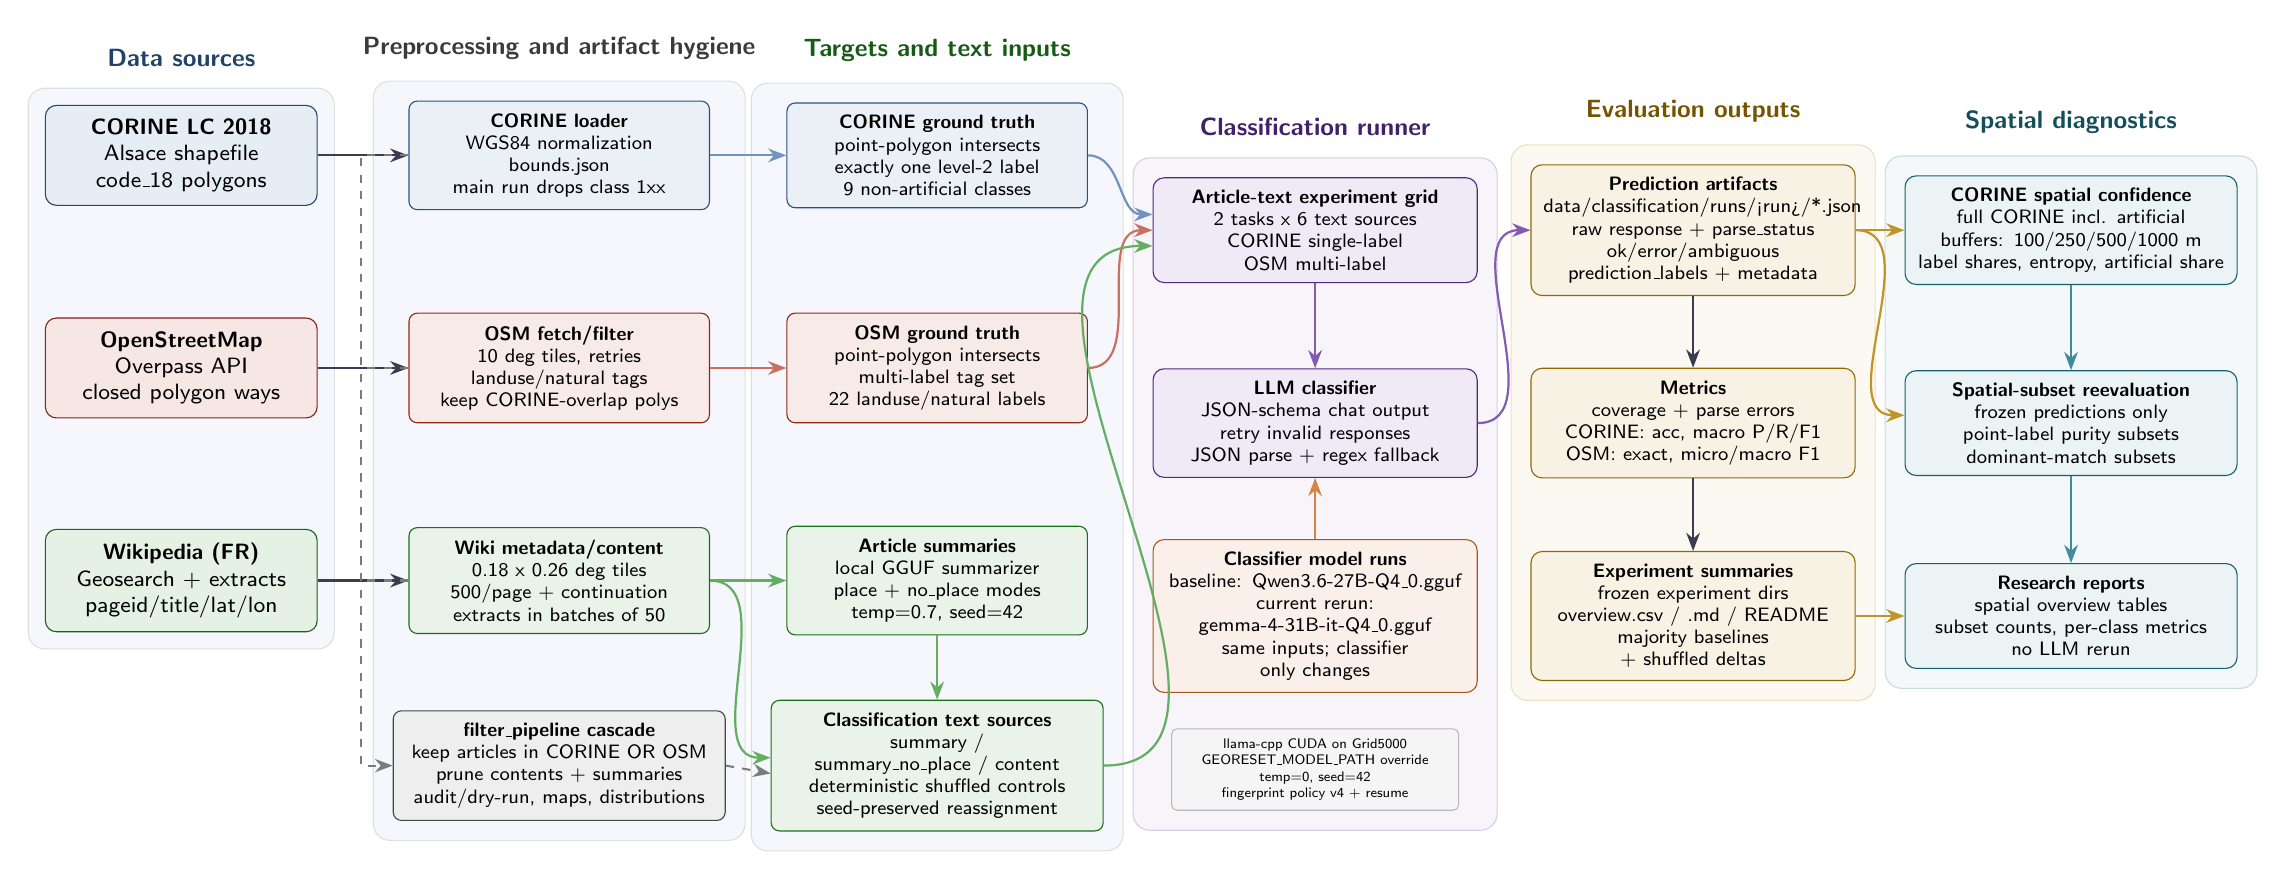
\begin{tikzpicture}[x=1cm,y=1cm]

%% ============================================================
%% COLUMN 1 - DATA SOURCES (x=0)
%% ============================================================
\node[datasrc=clcblue] (clc) at (0,3.4)
  {\textbf{CORINE LC 2018}\\Alsace shapefile\\code\_18 polygons};

\node[datasrc=osmred] (osm) at (0,0.7)
  {\textbf{OpenStreetMap}\\Overpass API\\closed polygon ways};

\node[datasrc=wikigreen] (wiki) at (0,-2.0)
  {\textbf{Wikipedia (FR)}\\Geosearch + extracts\\pageid/title/lat/lon};

%% ============================================================
%% COLUMN 2 - DATA PREP AND FILTERS (x=4.8)
%% ============================================================
\node[process=clcblue] (clcprep) at (4.8,3.4)
  {\textbf{CORINE loader}\\WGS84 normalization\\bounds.json\\main run drops class 1xx};

\node[process=osmred] (osmprep) at (4.8,0.7)
  {\textbf{OSM fetch/filter}\\10 deg tiles, retries\\landuse/natural tags\\keep CORINE-overlap polys};

\node[process=wikigreen] (wikiprep) at (4.8,-2.0)
  {\textbf{Wiki metadata/content}\\0.18 x 0.26 deg tiles\\500/page + continuation\\extracts in batches of 50};

\node[wideprocess=filtergray] (cascade) at (4.8,-4.35)
  {\textbf{filter\_pipeline cascade}\\keep articles in CORINE OR OSM\\prune contents + summaries\\audit/dry-run, maps, distributions};

%% ============================================================
%% COLUMN 3 - TEXTS AND TARGETS (x=9.6)
%% ============================================================
\node[process=clcblue] (gtcorine) at (9.6,3.4)
  {\textbf{CORINE ground truth}\\point-polygon intersects\\exactly one level-2 label\\9 non-artificial classes};

\node[process=osmred] (gtosm) at (9.6,0.7)
  {\textbf{OSM ground truth}\\point-polygon intersects\\multi-label tag set\\22 landuse/natural labels};

\node[process=wikigreen] (summaries) at (9.6,-2.0)
  {\textbf{Article summaries}\\local GGUF summarizer\\place + no\_place modes\\temp=0.7, seed=42};

\node[wideprocess=wikigreen] (texts) at (9.6,-4.35)
  {\textbf{Classification text sources}\\summary / summary\_no\_place / content\\deterministic shuffled controls\\seed-preserved reassignment};

%% ============================================================
%% COLUMN 4 - EXPERIMENT RUNNER AND MODELS (x=14.4)
%% ============================================================
\node[taskbox=llmviolet] (grid) at (14.4,2.45)
  {\textbf{Article-text experiment grid}\\2 tasks x 6 text sources\\CORINE single-label\\OSM multi-label};

\node[taskbox=llmviolet] (classifier) at (14.4,0.0)
  {\textbf{LLM classifier}\\JSON-schema chat output\\retry invalid responses\\JSON parse + regex fallback};

\node[taskbox=gemmaorange] (models) at (14.4,-2.45)
  {\textbf{Classifier model runs}\\baseline: Qwen3.6-27B-Q4\_0.gguf\\current rerun: gemma-4-31B-it-Q4\_0.gguf\\same inputs; classifier only changes};

\node[notebox] (runmeta) at (14.4,-4.40)
  {llama-cpp CUDA on Grid5000\\GEORESET\_MODEL\_PATH override\\temp=0, seed=42\\fingerprint policy v4 + resume};

%% ============================================================
%% COLUMN 5 - OUTPUTS AND EVALUATION (x=19.2)
%% ============================================================
\node[metricbox] (preds) at (19.2,2.45)
  {\textbf{Prediction artifacts}\\data/classification/runs/<run>/*.json\\raw response + parse\_status\\ok/error/ambiguous\\prediction\_labels + metadata};

\node[metricbox] (metrics) at (19.2,0.0)
  {\textbf{Metrics}\\coverage + parse errors\\CORINE: acc, macro P/R/F1\\OSM: exact, micro/macro F1};

\node[metricbox] (overview) at (19.2,-2.45)
  {\textbf{Experiment summaries}\\frozen experiment dirs\\overview.csv / .md / README\\majority baselines + shuffled deltas};

%% ============================================================
%% COLUMN 6 - SPATIAL CONFIDENCE DIAGNOSTICS (x=24.0)
%% ============================================================
\node[diagbox] (spconf) at (24.0,2.45)
  {\textbf{CORINE spatial confidence}\\full CORINE incl. artificial\\buffers: 100/250/500/1000 m\\label shares, entropy, artificial share};

\node[diagbox] (speval) at (24.0,0.0)
  {\textbf{Spatial-subset reevaluation}\\frozen predictions only\\point-label purity subsets\\dominant-match subsets};

\node[diagbox] (reports) at (24.0,-2.45)
  {\textbf{Research reports}\\spatial overview tables\\subset counts, per-class metrics\\no LLM rerun};

%% ============================================================
%% BACKGROUND GROUPS
%% ============================================================
\begin{scope}[on background layer]
  \node[draw=gray!25, fill=boxbg, rounded corners=6pt,
        fit=(clc)(osm)(wiki), inner sep=6pt] (bg1) {};
  \node[draw=gray!25, fill=boxbg, rounded corners=6pt,
        fit=(clcprep)(osmprep)(wikiprep)(cascade), inner sep=7pt] (bg2) {};
  \node[draw=gray!25, fill=boxbg, rounded corners=6pt,
        fit=(gtcorine)(gtosm)(summaries)(texts), inner sep=7pt] (bg3) {};
  \node[draw=llmviolet!25, fill=llmviolet!5, rounded corners=6pt,
        fit=(grid)(classifier)(models)(runmeta), inner sep=7pt] (bg4) {};
  \node[draw=metricgold!25, fill=metricgold!5, rounded corners=6pt,
        fit=(preds)(metrics)(overview), inner sep=7pt] (bg5) {};
  \node[draw=diagcyan!25, fill=diagcyan!5, rounded corners=6pt,
        fit=(spconf)(speval)(reports), inner sep=7pt] (bg6) {};
\end{scope}

%% ============================================================
%% SECTION LABELS (Positioned relative to backgrounds)
%% ============================================================
\node[sectionlabel=clcblue, above=0.15cm of bg1] {Data sources};
\node[sectionlabel=filtergray, above=0.15cm of bg2] {Preprocessing and artifact hygiene};
\node[sectionlabel=wikigreen, above=0.15cm of bg3] {Targets and text inputs};
\node[sectionlabel=llmviolet, above=0.15cm of bg4] {Classification runner};
\node[sectionlabel=metricgold, above=0.15cm of bg5] {Evaluation outputs};
\node[sectionlabel=diagcyan, above=0.15cm of bg6] {Spatial diagnostics};

%% ============================================================
%% MAIN FLOW ARROWS
%% ============================================================
% Col 1 to Col 2
\draw[myarrow] (clc) -- (clcprep);
\draw[myarrow] (osm) -- (osmprep);
\draw[myarrow] (wiki) -- (wikiprep);

% Filter Cascade Bus (Dashed)
\draw[myarrowdashed, color=filtergray!80] (clcprep.west) -- ++(-0.6,0) coordinate (bus_top) -- (bus_top |- cascade.west) -- (cascade.west);
\draw[color=filtergray!80, dashed, thick] (osmprep.west) -- (osmprep.west -| bus_top);
\draw[color=filtergray!80, dashed, thick] (wikiprep.west) -- (wikiprep.west -| bus_top);

% Col 2 to Col 3
\draw[myarrow, color=clcblue!70] (clcprep.east) -- (gtcorine.west);
\draw[myarrow, color=osmred!70] (osmprep.east) -- (gtosm.west);
\draw[myarrow, color=wikigreen!70] (wikiprep.east) -- (summaries.west);

\draw[myarrow, color=wikigreen!70] (summaries.south) -- (texts.north);
\draw[myarrow, color=wikigreen!70] (wikiprep.east) to[out=0,in=180] ([yshift=0.1cm]texts.west);
\draw[myarrowdashed, color=filtergray!80] (cascade.east) -- ([yshift=-0.1cm]texts.west);

% Col 3 to Col 4
\draw[myarrow, color=clcblue!70] (gtcorine.east) to[out=0,in=180] ([yshift=0.2cm]grid.west);
\draw[myarrow, color=osmred!70] (gtosm.east) to[out=0,in=180] (grid.west);
\draw[myarrow, color=wikigreen!70] (texts.east) to[out=0,in=180] ([yshift=-0.2cm]grid.west);

% Inside Col 4
\draw[myarrow, color=llmviolet!80] (grid.south) -- (classifier.north);
\draw[myarrow, color=gemmaorange!85] (models.north) -- (classifier.south);

% Col 4 to Col 5
\draw[myarrow, color=llmviolet!80] (classifier.east) to[out=0,in=180] (preds.west);
\draw[myarrow] (preds.south) -- (metrics.north);
\draw[myarrow] (metrics.south) -- (overview.north);

% Col 5 to Col 6
\draw[myarrow, color=metricgold!85] (preds.east) -- (spconf.west);
\draw[myarrow, color=diagcyan!85] (spconf.south) -- (speval.north);
\draw[myarrow, color=metricgold!85] (preds.east) to[out=0,in=180] ([yshift=0.1cm]speval.west);
\draw[myarrow, color=diagcyan!85] (speval.south) -- (reports.north);
\draw[myarrow, color=metricgold!85] (overview.east) -- (reports.west);

\end{tikzpicture}
\end{document}
